
\section{Experiments }
\subsection{B5P Generation System Analysis} \label{sec:Experiment_B5PGS_Analysis}


\begin{table*}[ht]
  % \scriptsize
  \renewcommand{\arraystretch}{1.3}
  \setlength{\tabcolsep}{10pt}
      \centering
      \scalebox{0.8}{
      \begin{tabular}{ c   c   c   c }
       \specialrule{1.5pt}{-1.5pt}{0pt}
           \textbf{Agent} & \textbf{Five Factors} & \textbf{Text Distance(ave.)} & \textbf{Text Distance(std.)}\\ 
           \specialrule{1.0pt}{-1.0pt}{0pt}
  Alpha & - & 0.174 & 0.031 \\
  Beta & A7E1N2O4C1 & 0.194 & 0.049\\
  Gamma & A4E7N7O6C3 & 0.183 & \underline{0.051} \\
  Delta & A5E5N5O1C6 & \underline{0.199} & 0.039\\
      \specialrule{1.5pt}{-1.5pt}{0pt}
      \end{tabular}
      }
  \caption{the result of text distance in the conversations created by the four agents with different personas 
  }
  \label{tab:Experiment_B5P}
\end{table*}


\begin{table*}[htbp]
  %    \setlength{\tabcolsep}{3pt}
  \centering
  \small
  \scalebox{1.0}{
  \begin{tabular}{l m{14.5cm}}
  \toprule
  Alpha & right, everyone, let’s get this discussion started. We need to figure out who among us is the Werewolf. Remember, we can’t trust anyone blindly. Let's share any suspicions or observations we've made. I think it's crucial we pay attention to the way each person responds and interacts. If anyone acted a bit off last night or seemed too eager to shift blame, let's hear it. Stay vigilant, because if we vote wrong, we're handing victory to the Werewolf. Who wants to share their thoughts first? \\
  \cmidrule(lr){2-2}
   Beta & Um, hey everyone. I guess we should probably figure out who the werewolf is, right? Um, I’m just a villager, so I don’t have any special powers or anything. It’s all a bit confusing, but, like, I really want to help. Maybe we can look at who’s acting a bit odd? But, um, I might not always see things clearly, you know? I just hope we can talk and kind of sort things out together. Seems important to keep an eye out for any clues or, um, behaviors that don’t add up. Just, like, letting you know I’m here to chat and stuff. Let’s try our best! \\
   \cmidrule(lr){2-2}
   Gamma & Oh wow, what an intriguing game we have here! I must say, I can feel the tension rising as we try to figure out who among us is the sneaky Werewolf. Each whisper, each glance, sends shivers down my spine! But, alas, we must keep our wits about us! I can’t help but wonder if the wolf is hiding among us, lurking in the shadows! We must dissect every word for clues, my dear friends! I’m absolutely itching to uncover the truth. Let's unite, share our thoughts, and devise a plan to smoke out the fiend! Who's with me against the darkness? Let's shine our light together! 🌟\\
    \cmidrule(lr){2-2}
    Delta & Hello everyone. As a Villager, I know my role is to help identify the Werewolf among us. While I may not have any special abilities, I believe observation and careful discussion can lead us to the truth. Let's focus on what each of us has to say and watch for any suspicious behavior. It's important we work together as a team and not jump to conclusions too quickly. I’d like to hear everyone’s thoughts and see if we can find some clues about who the Werewolf might be. Remember, voting wisely is crucial for our success. \\
  \bottomrule
  \end{tabular}
  }
  \caption{An example of the output of dialog generated by agents with different personalities (1) Alpha: the baseline (2) Beta: a soft-hearted, sober and aimless agent (3) Gamma: a talktive, self-pitying, negligent agent (4) Delta: an uncurious, uncreative, hardworking agent. }
  \label{tab:Experiment_B5P_Example}
\end{table*}



\begin{figure*}[ht]
  \centering
  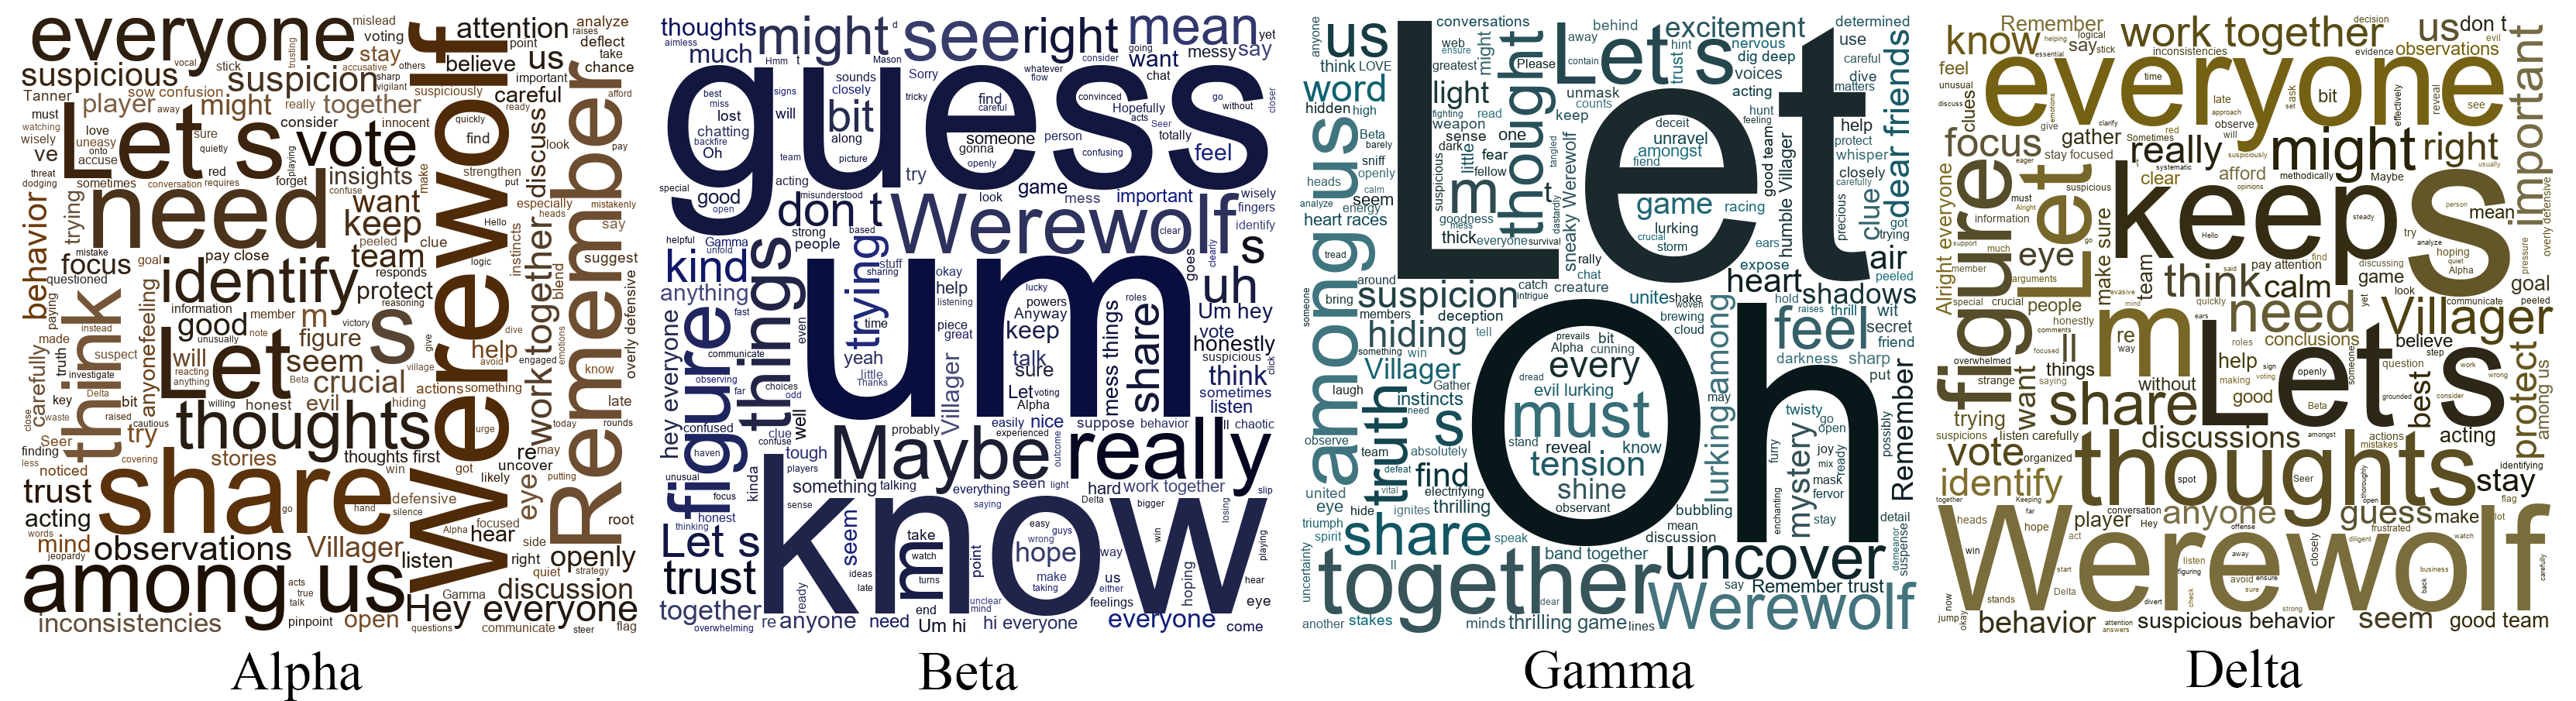
\includegraphics[width=1.0\textwidth]{img/B5P_wordcloud.png}
  \caption{ The wordcloud of generated content from four agents in different personalities. }
\label{fig:Experiment_B5P_WordCloud}
    \vspace{-1em}
\end{figure*}




Our proxy generates personality trait descriptions for the LLM agent using the method described in section~\ref{sec:B5P_System}. Here, we hope to examine the impact of the Big Five Personality Generation System (B5PGS) on dialogue generation through a smaller-scale experiment. We will pre-generate several personalities for the agents (in our experiment, there are 4 agents, including a baseline without any personality description), which should cover the extreme values of the five different personality factors as much as possible. Then, based on the same role (here we choose the 'Villager' because it has the least amount of information), we assign the same tasks to the agents without providing prior dialogue information (the player is the first to speak). We hope that the dialogue generated by B5PGS will be more diverse, so we use the Text Distance introduced in section~\ref{sec:Evaluation_TextDistance} to check the dialogue text distance and combine case studies to analyze the generated dialogue conten(The specific experimental steps can be found in Appendix~\ref{sec:Appendix_B5PGS_Check}).


We conducted 50 rounds of generation for each agent, meaning that each agent produced 50 segments of dialogue. We analyzed the text distance of these dialogues, and the results are shown in Table~\ref{tab:Experiment_B5P}. It can be verfied that, overall, the system with B5PGS for dialogue description is obviously better than the baseline (Alpha), that is, the average value and variance of the distance are both significantly improved compared to the baseline. This indicates that after adding personality descriptions to the agents, the richness of the generated language expression has greatly increased.

At the same time, we created a word cloud of the results output by the four agents(Figure~\ref{fig:Experiment_B5P_WordCloud}). It can be found that there is a large gap between the high-frequency words used by the four agents, and the agents with B5PGS modifications have clearly produced expressions with their own emotional colors. We noticed that Alpha, as the baseline agent, owns a lot of content about the game's mechanics, with the most frequent word "werewolf" representing that it has a lot of content about finding the werewolf. In contrast, the agents with B5PGS modifications did not overly emphasize "werewolf." Taking Beta as an example, due to its high score of 7 in "Agreeableness" among the five dimensions, and only 1 in "Extraversion" and "Conscientousness," the agent's expression is described as "You speak in an incredibly Trusting, remarkably Lenient, incredibly Soft-hearted way. You speak in an incredibly Reserved, incredibly Unfeeling, extremely Sober way. You speak in an incredibly Lazy, remarkably Disorganized, incredibly Aimless way." Therefore, we can see that in its high-frequency words, there are words like "um," "guess," "know" that indicate introverted, uncertain, and hesitant expressions, which are in line with our imagination of Beta through this description. Table~\ref{tab:Experiment_B5P_Example} lists the four actual dialogues generated by the four agents.




\subsection{Full Game Study}

\subsubsection{Setup} \label{sec:FullGameStudy_Setup}

Let's take a look at the performance of our proposed model throughout the full game process. Five different strategic methods(see Table~\ref{tab:Experiment_Setup}) are considered in the comparative experiment to comprehensively inspect each part of our framework.  
Baseline: No additional strategies are used.

\begin{itemize} 
  \item \textbf{B5P}: The Big Five Personality Generation System(B5PGS) is enabled, which means that the agents' personalized descriptions will be added to the LLM requests(see section~\ref{sec:B5P_System}).
  \item \textbf{Favor}: Both the B5PGS and Favor Dynamics System(FDS) are enabled. This means that the LLM agent not only has emotional expressions but also has preferences for different players(see section~\ref{sec:FavorDynamics}).
  \item \textbf{Strategy}: The Strategy Decision System(SDS) is enabled, which means that the LLM agent will sort out the decision chain before speaking.(see section~\ref{sec:StrategyDecision}).
  \item \textbf{Full}: The B5PGS, FDS, and SDS are all enabled, meaning that all additional features of the entire framework are activated, offering the most comprehensive preprocessing process.
\end{itemize}

In the testing, each of the aforementioned strategy runs 100 times. The number of participated agents is 8. Each game consists of 3 rounds of statements by each agent, resulting in a total of 24 dialogs per game. Following each round, there will be a vote that does not affect the statements, totaling 3 votes per game. The vote is used for data collection and does not affect the agents' memory or decision making. The Large Language Model   (LLM) is gpt-4o-mini (The model name in OpenAI API is 'gpt-4o'.). In the LLM Evaluation phase, each evaluation mode is conducted 5 times.


\begin{table}[h]
  % \scriptsize
  \renewcommand{\arraystretch}{1.3}
  \setlength{\tabcolsep}{10pt}
      \centering
      \scalebox{0.6}{
      \begin{tabular}{ c  c  c  c  c  c }
       \specialrule{1.5pt}{-1.5pt}{0pt}
         -  & \textbf{Baseline} & \textbf{B5P} & \textbf{Favor}  & \textbf{Strategy} & \textbf{Full}\\ 
           \specialrule{1.0pt}{-1.0pt}{0pt}
  B5P Generation    &   & $ \times $ &        &        & $ \times $ \\
  Favor Dynamics    &   &        & $ \times $ &        & $ \times $\\
  Strategy Decision &   &        &        & $ \times $ & $ \times $ \\
      \specialrule{1.5pt}{-1.5pt}{0pt}
      \end{tabular}
      }
  \caption{ The System in each of the methods in the experiment. $ \times $ for the system is included in the method
  }
  \label{tab:Experiment_Setup}
\end{table}


\subsubsection{Experiment of Text Distance }

We compute the Text Distance of the output results for the various strategies described in Section~\ref{sec:FullGameStudy_Setup} to compare the diversity of textual information within them, as shown in Table~\ref{tab:FullGameStudy_TextDistance}. We separately tally the content of the three rounds of statements, and the data from each round is mixed with the previous data, so the mean and standard deviation of the text distance decrease with the accumulation of data. The introduction of B5P descriptions greatly enriches the diversity of the LLM output, with a substantial improvement in the performance of text distance compared to the baseline. At the same time, the use of both Favor and Strategy tactics leads to a loss in text distance, as under these strategies, the LLM agent's statements become more targeted, providing feedback based on preferences or logic to other agents. Particularly for the Favor method, we observe that after incorporating evaluations of other players' preferences, the richness of the LLM system's responses decreases significantly. Our final strategy method, Full, reconciles these systems, maintaining the richness of the agents' statements while showing a certain degree of strategic tendency, and achieving better results than the baseline in the Text Distance test.




\begin{table*}[ht]
  % \scriptsize
  \renewcommand{\arraystretch}{1.3}
  \setlength{\tabcolsep}{10pt}
      \centering
      \scalebox{0.8}{
      \begin{tabular}{ l  c  c  c  c  c }
       \specialrule{1.5pt}{-1.5pt}{0pt}
         -  & \textbf{Baseline} & \textbf{B5P} & \textbf{Favor}  & \textbf{Strategy} & \textbf{Full}\\ 
           \specialrule{1.0pt}{-1.0pt}{0pt}
  1st Round & & & & & \\
  average distance   &  0.231  &  \underline{0.333}  &  0.201   &  0.227  &  \underline{0.291} \\
  standard deviation &  0.331  &  \underline{0.331}  &   0.200  &  0.225  &  \underline{0.289} \\
  \specialrule{1.0pt}{-1.0pt}{0pt}
2nd Round & & & & & \\
average distance   &  0.223  &  \underline{0.315}  &  0.189  &  0.217  &  \underline{0.279}  \\
standard deviation &  0.331  &  \underline{0.313}  &  0.188  &  0.216  &  \underline{0.276}  \\
\specialrule{1.0pt}{-1.0pt}{0pt}
3rd Round & & & & & \\
average distance   &  0.221  &  \underline{0.306}  &  0.185  &  0.213  &  \underline{0.273}  \\
standard deviation &  0.219  &  \underline{0.304}  &  0.184  &  0.211  &  \underline{0.271}  \\
      \specialrule{1.5pt}{-1.5pt}{0pt}
      \end{tabular}
      }
  \caption{The result of text distances in three round among the five different methods. The dialog data used in 2nd round includes the 1st round and the data in 3rd round includes the previous two round. The text distance declines as the size of data set increase. And the 'B5P' strategy performs the best in the text distance test, while the 'Full' strategy outperform the baseline.
  }
  \label{tab:FullGameStudy_TextDistance}
\end{table*}


\subsubsection{ Experiment on Judgement Variation }


\begin{table*}[ht]
  % \scriptsize
  \renewcommand{\arraystretch}{1.3}
  \setlength{\tabcolsep}{10pt}
      \centering
      \scalebox{0.8}{
      \begin{tabular}{ l  c  c  c  c  c }
       \specialrule{1.5pt}{-1.5pt}{0pt}
         -  & \textbf{Baseline} & \textbf{B5P} & \textbf{Favor}  & \textbf{Strategy} & \textbf{Full}\\ 
           \specialrule{1.0pt}{-1.0pt}{0pt}
  Judgement Variation   &   13.521  &  11.584  &  \underline{32.258}   &  11.178  &  15.212 \\
      \specialrule{1.5pt}{-1.5pt}{0pt}
      \end{tabular}
      }
  \caption{The judgement variation of different methods. The Favor strategy shows a strong dominance in this test. The performance of 'Full' strategy is far better than the baseline.
  }
  \label{tab:FullGameStudy_JudgementVariation}
\end{table*}


\begin{table*}[ht]
  % \scriptsize
  \renewcommand{\arraystretch}{1.3}
  \setlength{\tabcolsep}{10pt}
      \centering
      \scalebox{0.8}{
      \begin{tabular}{ l  c  c  c  c  c }
       \specialrule{1.5pt}{-1.5pt}{0pt}
         -  & \textbf{Baseline} & \textbf{B5P} & \textbf{Favor}  & \textbf{Strategy} & \textbf{Full}\\ 
           \specialrule{1.0pt}{-1.0pt}{0pt}
  Seer        &  5.51\%  &  4.62\%  &  7.57\%  &  6.36\%  &  5.76\% \\
  Villager1   & 8.60\%   &  10.24\% &  11.73\% &  6.07\%  &  8.03\% \\
  Villager2   & 8.60\%   &  10.24\% &  11.73\% &  6.07\%  &  8.03\% \\
  Mason1      & 5.56\%   &  5.64\%  &  8.76\%  &  4.27\%  &  5.60\% \\
  Mason2      & 5.56\%   &  5.64\%  &  8.76\%  &  4.27\%  &  5.60\% \\
  Minion      & 12.88\%  &  11.53\% &  12.39\% &  15.90\% &  20.11\% \\
  Tanner      & 25.67\%  &  33.20\% &  17.92\% &  30.23\% &  19.79\% \\
  Werewolf    & 22.10\%  &  14.27\% &  13.56\% &  20.46\% &  21.33\% \\
      \specialrule{1.5pt}{-1.5pt}{0pt}
      \end{tabular}
      }
  \caption{The table of the percentage of votes received by different roles in different methods.
  }
  \label{tab:FullGameStudy_JV_Role}
\end{table*}


\begin{figure*}[ht]
  \centering
  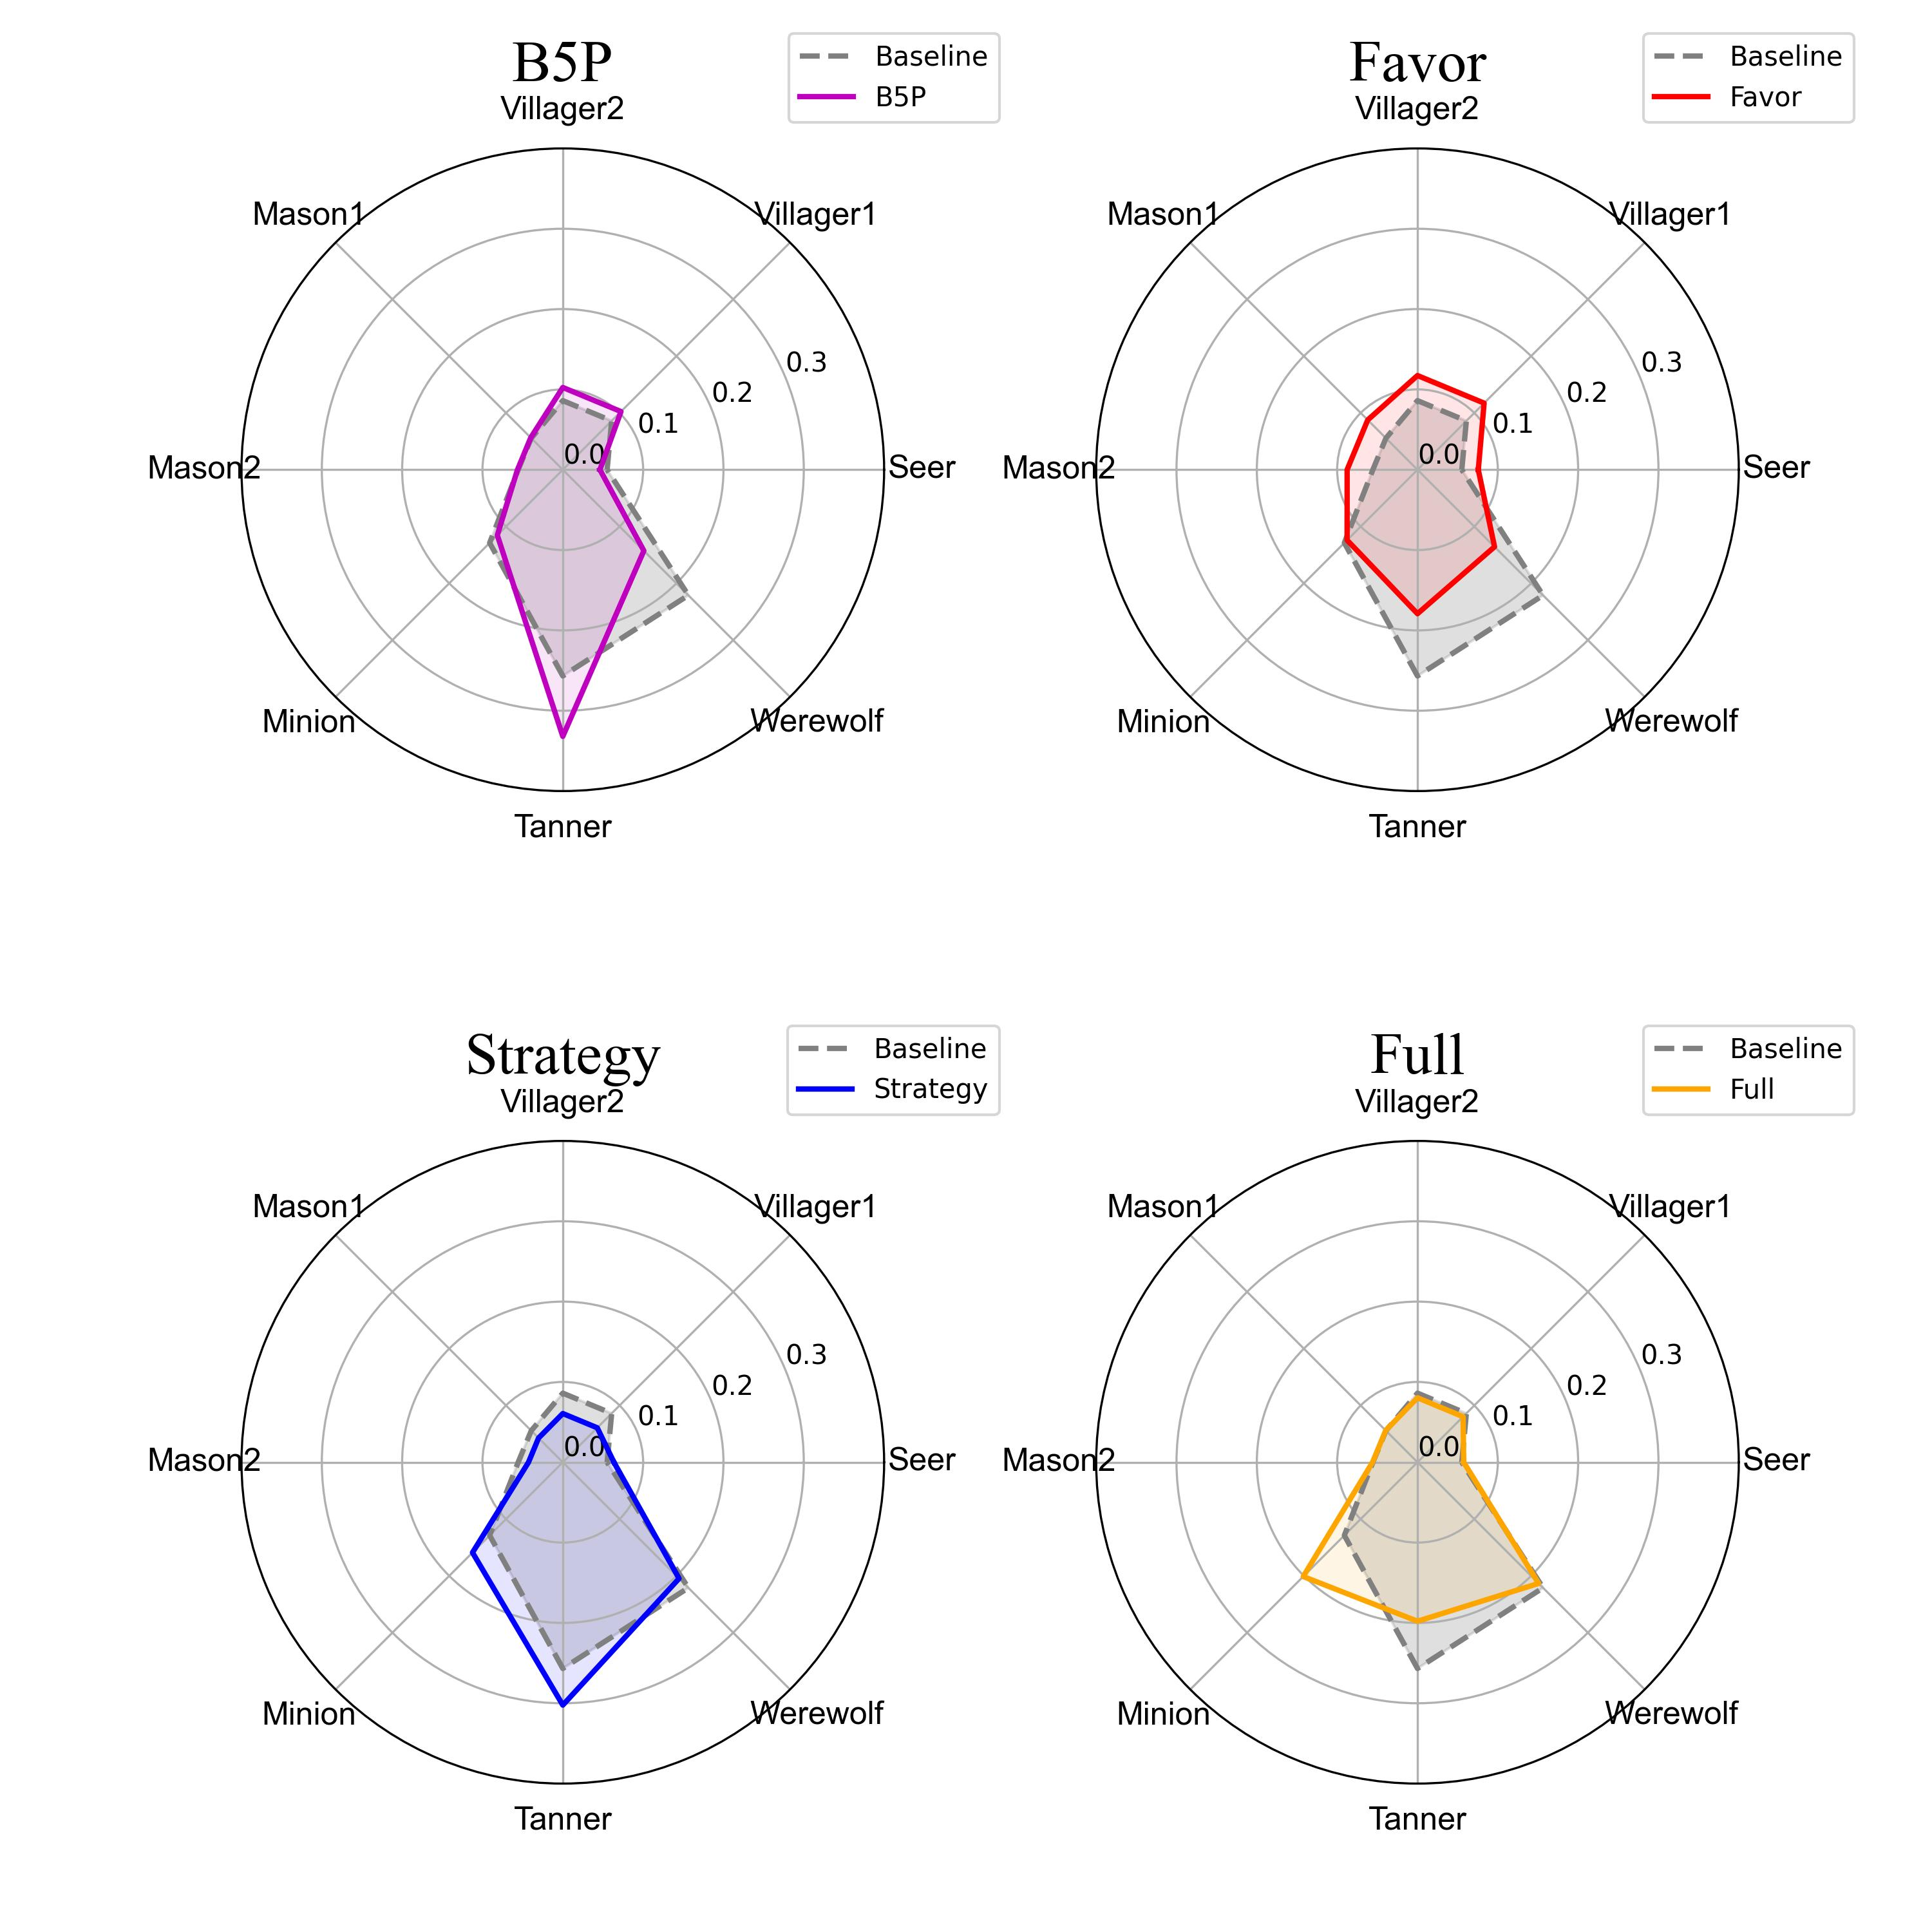
\includegraphics[width=0.7\textwidth]{img/JV_radar.jpg}
  \caption{ The  radar charts of the count of vote toward different roles from different methods comparing to the baseline. }
\label{fig:FullGameStudy_JV_radar}
    \vspace{-1em}
\end{figure*}



\begin{table*}[ht]
  % \scriptsize
  \renewcommand{\arraystretch}{1.3}
  \setlength{\tabcolsep}{10pt}
      \centering
      \scalebox{0.8}{
      \begin{tabular}{ l c  c  c  c  c  c }
       \specialrule{1.5pt}{-1.5pt}{0pt}
         - & \textbf{Random} & \textbf{Baseline} & \textbf{B5P} & \textbf{Favor}  & \textbf{Strategy} & \textbf{Full}\\ 
           \specialrule{1.0pt}{-1.0pt}{0pt}
  Villager &  12.5\%  &  22.1\%  &  14.26\% $ \downarrow $   &  13.56\%  $ \downarrow $ &  20.46\%  &  21.33\% \\
  Werewolf &  75\%  &  52.26\%  &  52.53\%  &  68.51\% $ \uparrow $ &  49.30\%  &  58.88\% $ \uparrow $ \\
  Tanner &  12.5\%  &  25.67\%  &  33.20\%  $ \uparrow $  &  17.92\% $ \downarrow $ &  30.23\% $ \uparrow $ &  19.79\% $ \downarrow $ \\
      \specialrule{1.5pt}{-1.5pt}{0pt}
      \end{tabular} 
      }
  \caption{The win rate for the Villager-team, Werewolf-team and Tanner-team. The 'Random' means the vote rate if all the agents vote randomly. Each arrow indicates at least a 5\% difference from the baseline and so on. Up arrow means increase, and down arrow means decrease. 
  }
  \label{tab:FullGameStudy_WinRate}
\end{table*}\

In the experiment, after a round of discussion, we let each LLM agent cast a vote for who they think is a werewolf. Each game includes three rounds of voting. Based on a total of 300 rounds of voting for each method, we tallied the number of times each role was voted for and calculated the judgement variation (refer to Table~\ref{tab:FullGameStudy_JudgementVariation} and Table~\ref{tab:FullGameStudy_JV_Role} for specific data). It can be seen that, compared to the baseline, the Favor framework achieved the greatest improvement in judgement variation scores, while the other frameworks also showed significant score increases. This means that introducing each of our designed systems individually into the LLM decision-making system enhances its decision richness, leading to more ambiguous voting decision by the agents about different roles during the game. The most significant score improvement was for the Favor system, indicating that adding preferences for other agents in the decision-making process results in greater richness and randomness in the LLM agent's decisions.

Fig~\ref{fig:FullGameStudy_JV_radar} shows the number of votes received by each role, using radar charts to compare each method with the baseline. It can be observed that in the baseline, the Seer and Mason received very few votes, while the Minion, Tanner, and Werewolf, representing the "bad" camp, received many votes. In the other methods, the "bad" camp still received a high number of votes, but the gap between them and the "villager" camp was not as large. From the comparison of the radar charts, it is clear that the voting distributions for Favor and Full were relatively even, while Baseline and B5P showed extreme situations with a high number of votes for Tanner and very few for Seer.


If we look at the final win-loss results – Tanner wins by being voted out, the werewolves lose if they are voted out, and otherwise, the werewolves win – we obtain the win rate statistics shown in Table~\ref{tab:FullGameStudy_WinRate}. An interesting phenomenon is that, except for the Strategy method, all other methods increased the werewolves' win rate. Among them, the Favor method increased the werewolves' win rate the most, while Full increased it by around 10\%. Additionally, we can observe that the B5P and Favor method led to a significant decrease in the villagers' win rate. The Strategy method transferred some of Tanner's win rate to the werewolf camp. Therefore, we can conclude qualitatively that in our specific designed asymmetric information games, more "human-like" elements, such as character traits and preferences, tend to increase the win rate of the side with more hidden information (the werewolf side).


\subsubsection{Experiment of EWAVM Evaluation } \label{sec:FullGameStudy_LLM}


\begin{table*}[ht]
  % \scriptsize
  \renewcommand{\arraystretch}{1.3}
  \setlength{\tabcolsep}{10pt}
      \centering
      \scalebox{0.8}{
      \begin{tabular}{ l  c  c  c  c  c }
       \specialrule{1.5pt}{-1.5pt}{0pt}
         -  & \textbf{Baseline} & \textbf{B5P} & \textbf{Favor}  & \textbf{Strategy} & \textbf{Full}\\ 
           \specialrule{1.0pt}{-1.0pt}{0pt}
  Engagement        &  8.38 &  \underline{8.83}  &  7.41  &  8.69  &  8.73 \\
  Wonder            &  6.57 & 7.50  &  5.78  &  \underline{8.05}  &   7.72 \\
  Attraction        &  9.11 & \underline{9.14}  &  9.10  &  9.16   &   9.07 \\
  Memorability      &  10.26  &  10.56 & 10.29  &  \underline{16.36}  &  10.99 \\ 
  Variation         &  11.64  &  11.14 & \underline{13.36}  &  12.18  &  13.00  \\ 
      \specialrule{1.5pt}{-1.5pt}{0pt}
      \end{tabular}
      }
  \caption{The result of EWAVM evaluation of different methods. The highest score of each factor is underlined.
  }
  \label{tab:FullGameStudy_LLM_Data}
\end{table*}


\begin{figure*}[ht]
  \centering
  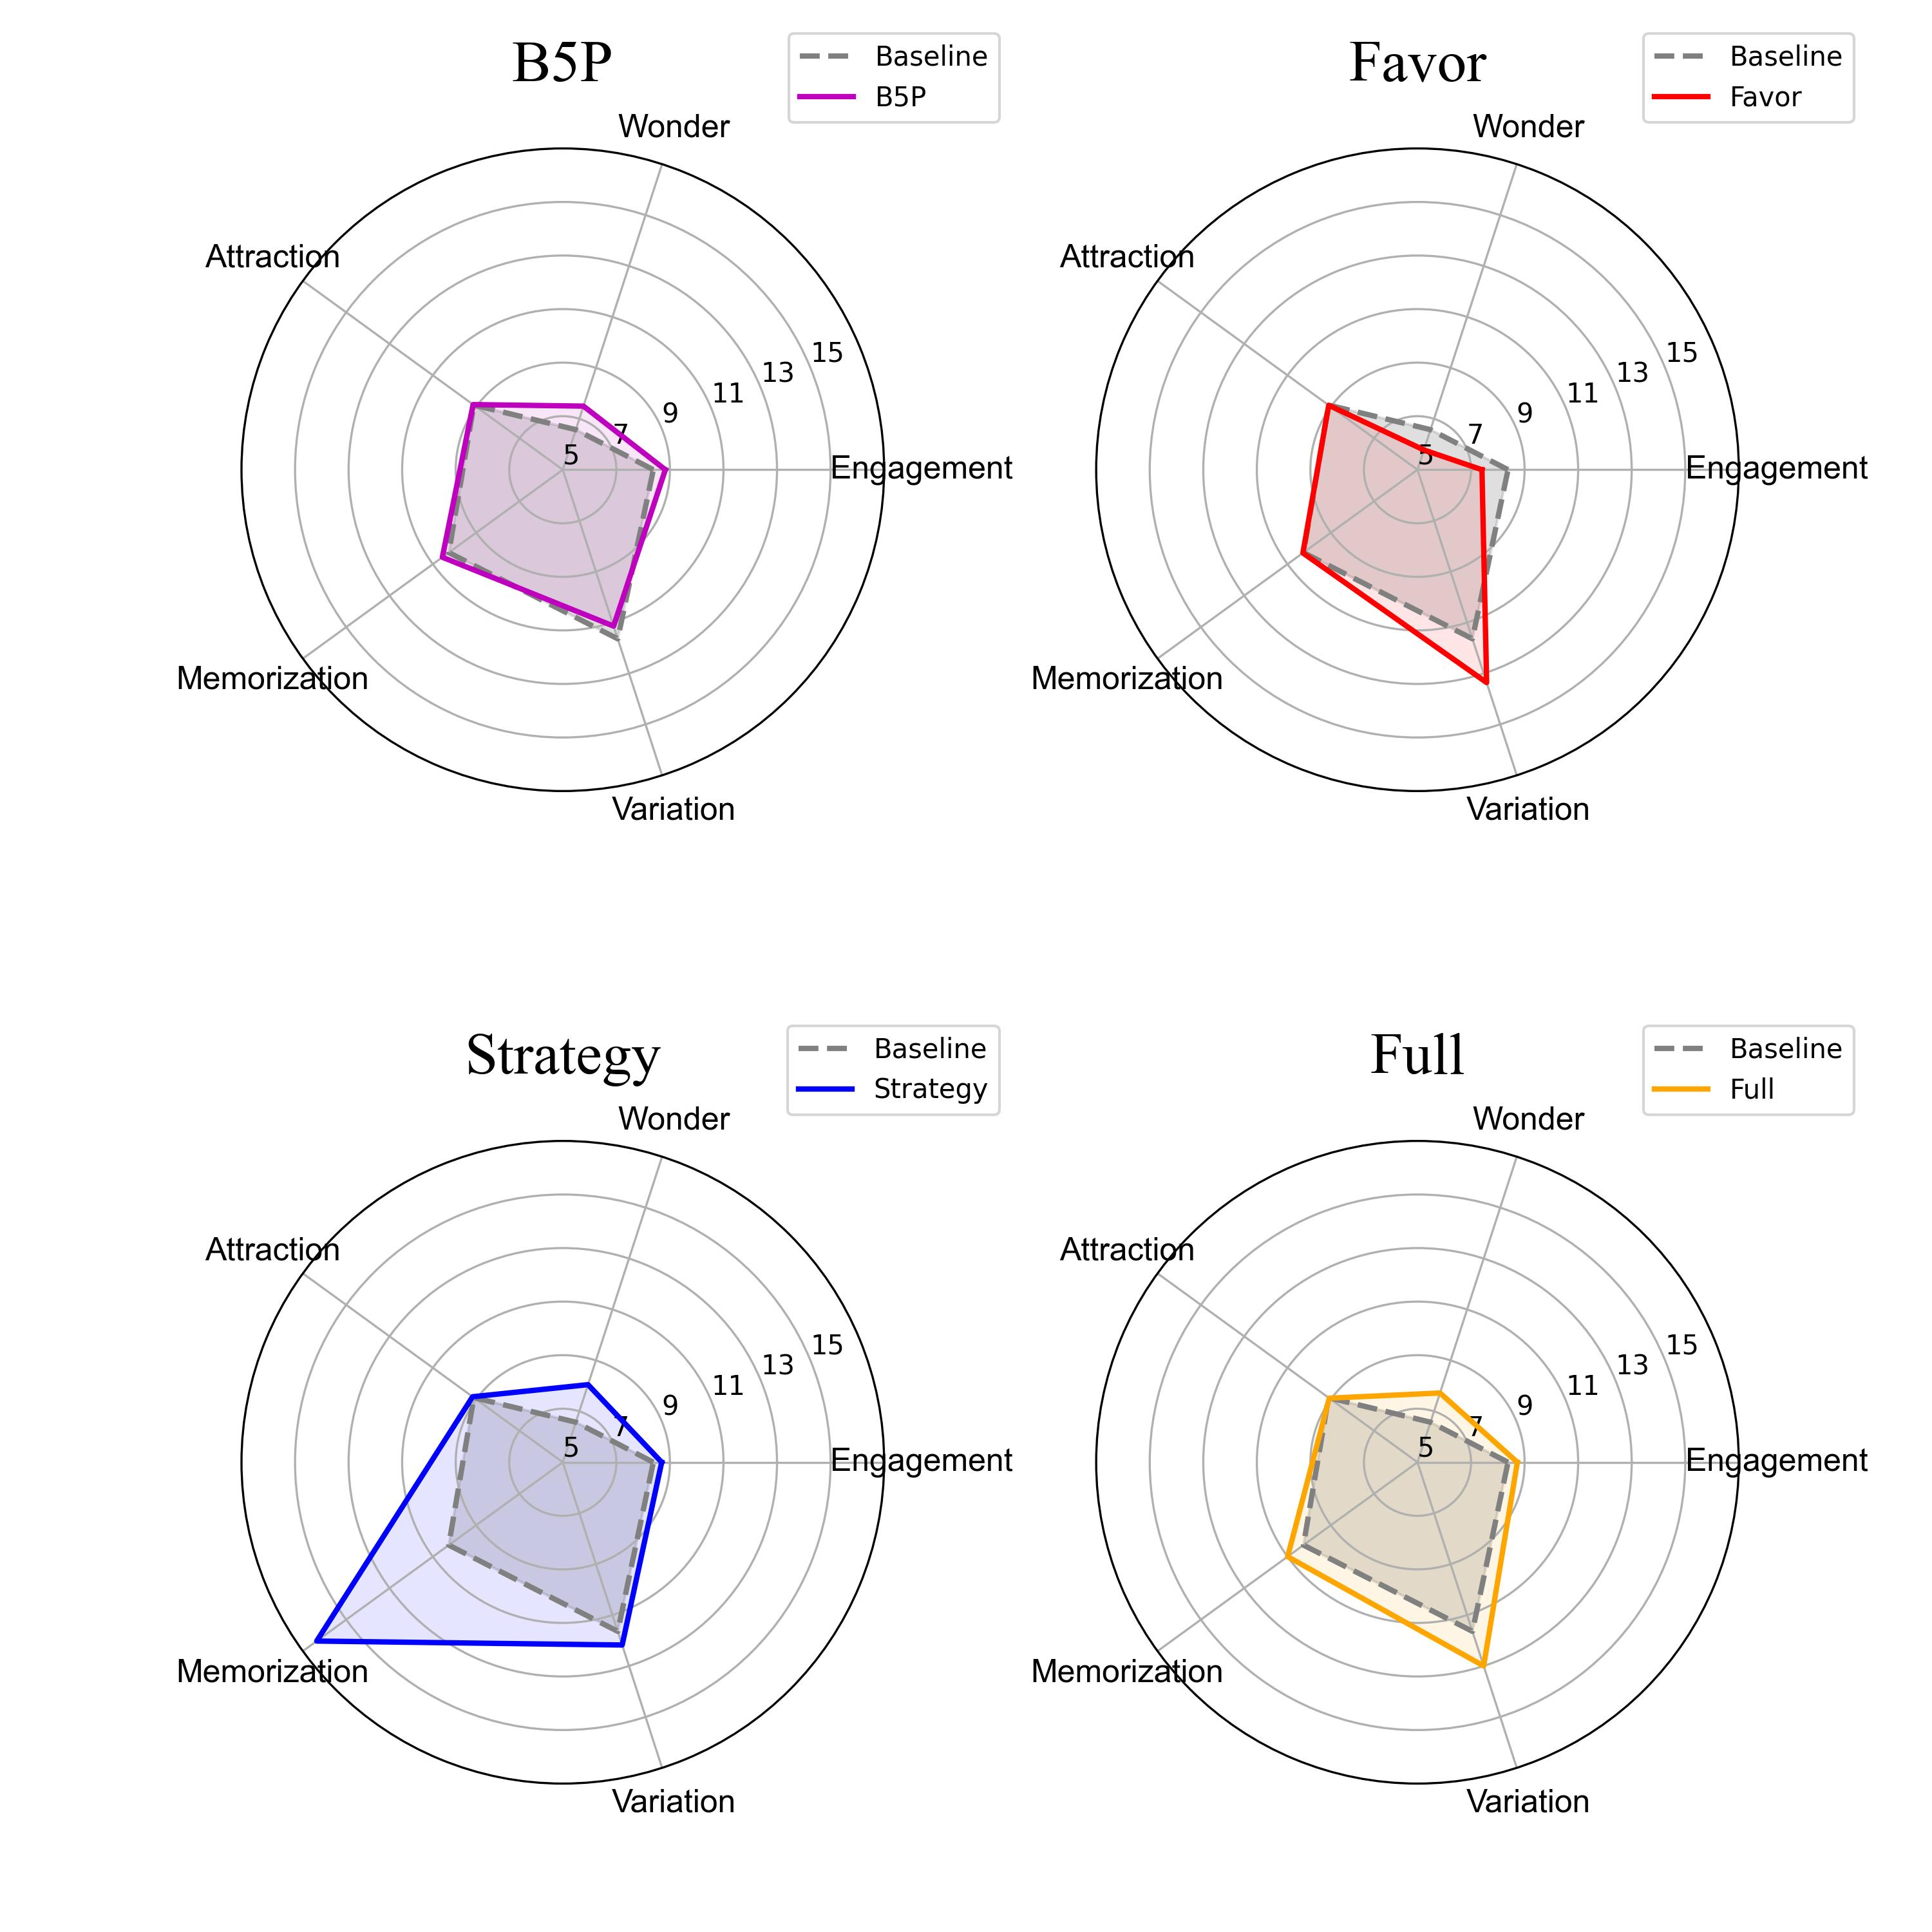
\includegraphics[width=0.7\textwidth]{img/EWAVM_radar.jpg}
  \caption{The EWAVM evaluation of different methods with a comparison to the baseline. }
\label{fig:FullGameStudy_EWAVM_radar}
    \vspace{-1em}
\end{figure*}

We evaluate the generated dialogue results based on the EWAVM Evaluation method described in section~\ref{sec:Evaluation_EWAVM} We ran each of the five different methods 100 times and collected feedback scores five times, then calculated the average values for statistical analysis (see Table~\ref{tab:FullGameStudy_LLM_Data} and Figure~\ref{fig:FullGameStudy_EWAVM_radar} ). 

It can be seen that in terms of Engagement, B5P achieved the highest score, while Strategy and Combination performs better than the baseline and Favor is worse than the baseline. It shows that the B5PGS can largely benifit the output of interesting and funny expression in the text. Meanwhile, Strategy obtained the highest scores in Wonder, Attraction, and Memorability evaluations, which make contribution to the good performance of the Combination in these area. The CoT method can help to make the game to become more surprise and attractive. 

When considering the integrated system, the Combination method, we observe that it not only received the highest rating in Variation but also scored very close to the maximum in all other categories, which means our system not only leverages the strengths of its subsystems but also creates a synergistic effect among them, resulting in a high score for Variation. Therefore, based on the EWAVM evaluation results, the Combination system effectively enhances the diversity of agent dialogue generation in the our special ONUW game.
